\subsubsection{UI components}\label{sec:ui-components}

Using components enabled me to split my \ac{UI}
into small, reusable components,
eliminating code duplication,
and helping with maintaining the consistent look.
I wanted to choose the right library
for this task,
so that the development would be quick,
and I would have plenty of tools
that would help me achieve
good architecture for the frontend.

\paragraph{UI component library}\label{sec:ui-component-library}

A \ac{UI} component library is a \acf{JS} or \acf{TS} library
enabling a programmer to reduce duplication
in the frontend codebase.
It provides a way to split the frontend code into components,
which can be parametrized, reused, and composed into an entire application,
and to declaratively describe
the appearance and behavior of those components
with a help of functions or classes.
When choosing the library for the \ac{UI} components, I considered:

\begin{itemize}
  \item
        React~\cite{oshannessy_react_2022},
  \item
        Vue.js~\cite{you_vuejs_2022}, and
  \item
        Angular~\cite{kalpakas_angular_2022}.
\end{itemize}

All those libraries are very popular,
so I chose React,
because I had the most experience with it in my professional work.

\paragraph{The component directory}\label{sec:the-component-directory}

All of the frontend components
are located in the component directory~\cite{sewera_notipie_2022-3}.
The directories are divided by category.
There are currently two categories,
\textit{canvas}, and
\textit{notification}.
Canvas category includes
an \texttt{AppCanvas} component,
responsible for displaying
a background in the right color,
and controlling the light or dark mode setting.
Notification category includes
a notification card,
a notification container,
which contains all the notifications
from the same App\footnote{
  The concept of an App is described
  in section~\ref{sec:app}.
}, and a notification board,
containing all the notifications
presented in the \ac{UI}.

\paragraph{Styling}\label{sec:ui-styling}

In addition to the correct behavior of the \ac{UI},
I needed to bring my design of the card\footnote{
  The design of the card
  is explained in detail
  in section~\ref{sec:final-design}.
} and other components
into reality.
I had some experience with Bootstrap~4~\cite{otto_bootstrap_2018},
but I did not like the look of it
and customizability was complicated.
I also had experience with plain \ac{CSS},
but I did not want additional hassle
of maintaining both \ac{JS} and \ac{CSS}.

I decided I will use a \ac{CSS} utility library,
which will remove additional effort
of manual \ac{CSS} management,
as well as provide me with the necessary tools
to implement my own, custom design.
Tailwind~CSS~\cite{wathan_tailwind_2022}
was my first and only choice.
Not only is it very popular,
but also the documentation is excellent,
there are many tutorials on YouTube,
and it was written by the authors
of \citetitle{wathan_refactoring_2018}~\cite{wathan_refactoring_2018},
one of the books that influenced
my style of design overall,
mentioned also in section~\ref{sec:inspirations}.

\paragraph{Testing}\label{sec:ui-testing}

\Ac{UI} visual testing tend to be very expensive,
both in terms of time and money.
I used Applitools Eyes~\cite{applitools_applitools_2022}
in my professional work,
and it was both slow,
and the tests were flaky.
I also did not want to spend any money
on the application development.

I used Jest~\cite{bekkhus_jest_2022} for unit tests,
and I was very content with it.
I found out that it has
a \textit{snapshot testing} capability~\cite{bekkhus_snapshot_2022}.
In addition to a \ac{CSS} utility library
like Tailwind~CSS,
I could be fairly sure
that if all \ac{HTML} classes stayed the same,
the look of the entire application
will stay the same.

The snapshot tests were very quick,
easy to review and debug,
whenever there was some unwanted change.
Coupled with Tailwind~CSS,
they provided a very powerful tool
for regression testing.

\paragraph{Storybook}\label{sec:storybook}

Another tool that helped with
component creation in isolation
was Storybook~\cite{shilman_storybook_2022}.
The isolation of components
helped with testing,
improved portability and reusability,
and helped me gather all the properties
of each component into an interactive
documentation.
It provided a convenient component library browser,
which worked both in dark and light mode.
The Storybook for Notipie is presented
for dark and light modes in
figures~\ref{fig:storybook-dark}
and~\ref{fig:storybook-light}
respectively.

\begin{figure}[p]
  \centering
  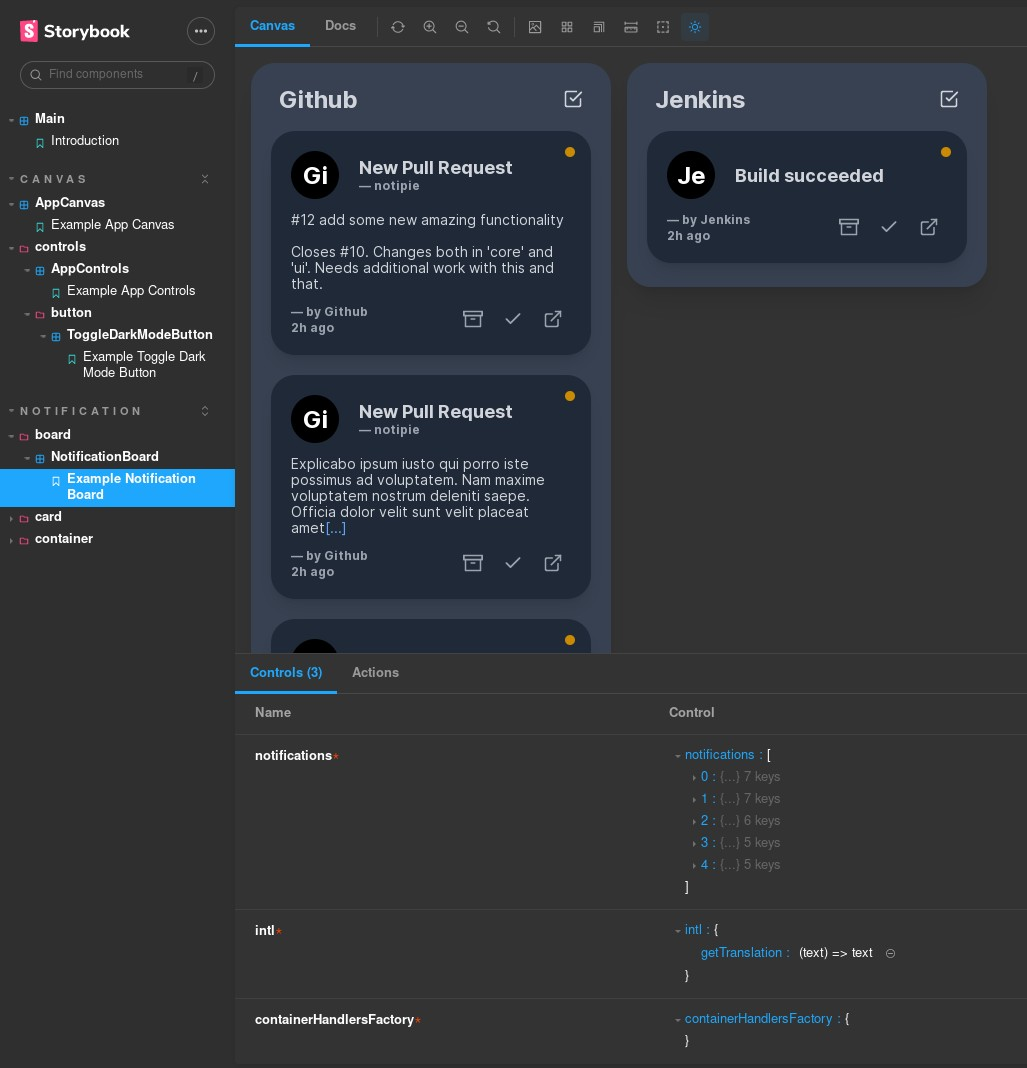
\includegraphics[width=\linewidth,keepaspectratio]{img/storybook.jpg}
  \caption{Storybook for Notipie: Dark mode view}
  \label{fig:storybook-dark}
\end{figure}

\begin{figure}[p]
  \centering
  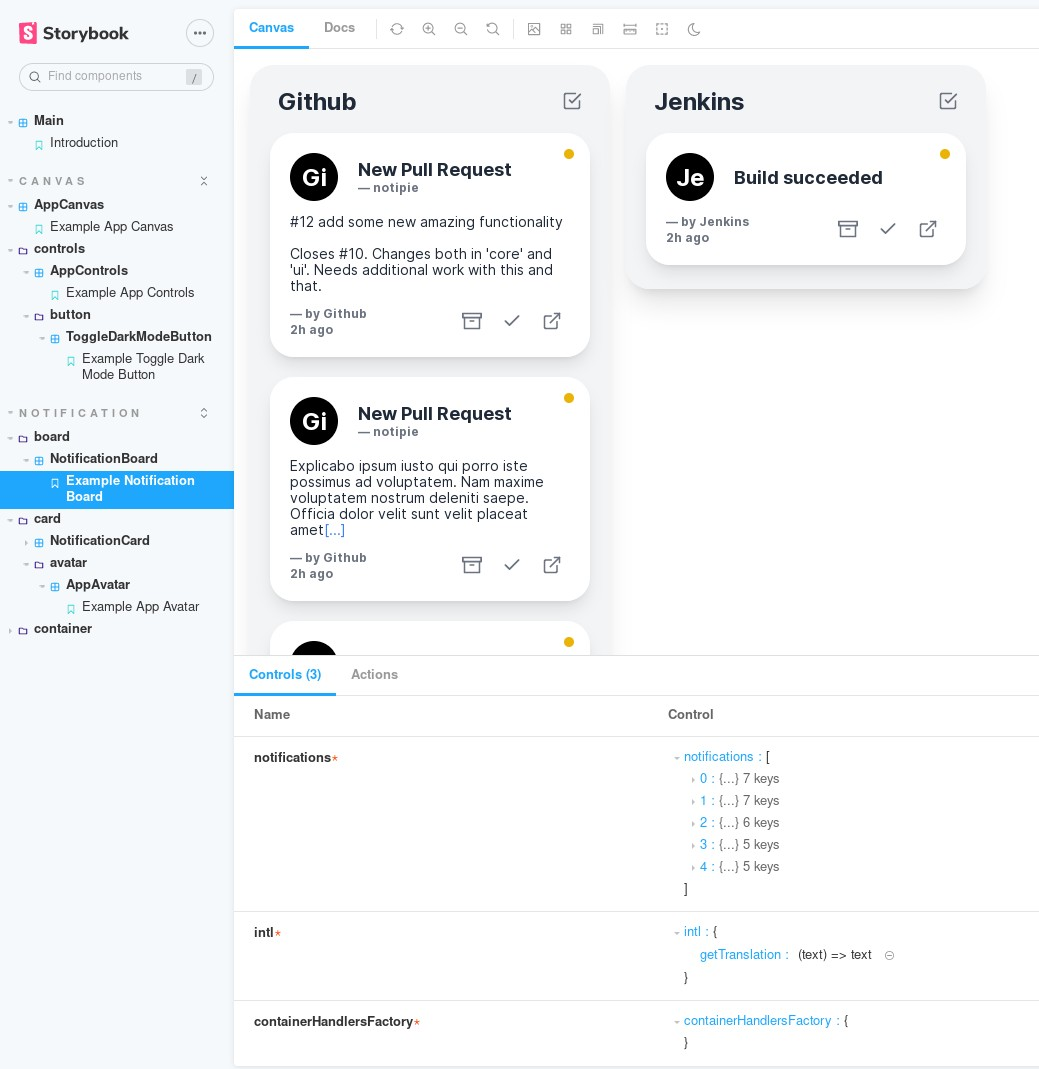
\includegraphics[width=\linewidth,keepaspectratio]{img/storybook_light.jpg}
  \caption{Storybook for Notipie: Light mode view}
  \label{fig:storybook-light}
\end{figure}
